\chapter{Test af reverb og echo impulsrespons}\label{sec:test_af_effekt}
Da echo og reverb begge er tidsinvariante effekter betyder det, at de kan karakteriseres af deres impulsrespons.\newline
Testens formål er at finde impulsresponset for echo- og reverbeffekten.
%Systemet består af modtager af indgangssignal, anti-aliasing filtre, TIVA-kit med EMP board, DAC, rekonstruktionsfilter og udgangskredsløbet.
Systemet består af et signalindgangs board, en række anti-aliasing og input filtre, et TIVA-kit med EMP board, et board med en DAC, nogle rekonstruktionsfilter og et udgangskredsløbet.
\section{Forsøgsopstilling og fremgangsmetode}
\begin{itemize}
	\item Funktionsgenerator sat på pulse med en peak-to-peak spænding sat til $500\si{mV}$ og et DC-offset sat til $250\si{mV}$ og pulsen sættes til at være $25\si{\mu S}$ lang svarende til en sample
	\item Oscilloskop sat til singe sweep med en trigger sat til $500\si{mV}$
	\item Load modstand koblet på udgangen på $10\si{k\Omega}$
	
	\husk{Sonny}{Er ikke sikke på at du har de rigtige værdier herunder, især fordi jeg måtte rette et par af dem ovenover}
	
	\item Reverb delay sat til $2000$ samples og input- og feedbackgain sat til $-0.45$
	\item Echo delay sat til $2000$ samples og gain sat til $0.5$
\end{itemize}
%Funktionsgeneratoren kobles på signalindgangen af systemet, og oscilloskopets prober placeres hhv. på indgangen til mikrocontrolleren og på udgangen af rekonstruktionsfilteret.\newline
Funktionsgeneratoren kobles på signalindgangen sammen med en af oscilloskopets prober, den anden placeres udgangskredsløbet.\newline
Effektmodulerne aktiveres hver for sig og der tages et single sweep.
\subsection{Resultat}
\husk{Sonny}{Samme input så det er ikke nødvendigt med to billeder blot en tekst der forklare at samme impuls blev anvendt}
\husk{Sonny}{Vi bør nok lige forbedre graferne, et screen grab ville eventuelt være en del bedre, ellers må vi selv lige tilføje de manglende detaljer eg. størrelsesorden og typer på akserne}
Inputtet til testene var for hhv. reverb og echotestene disse:
\begin{figure}[!ht]
		\centering
	\begin{minipage}{0.50\textwidth}
		\centering
		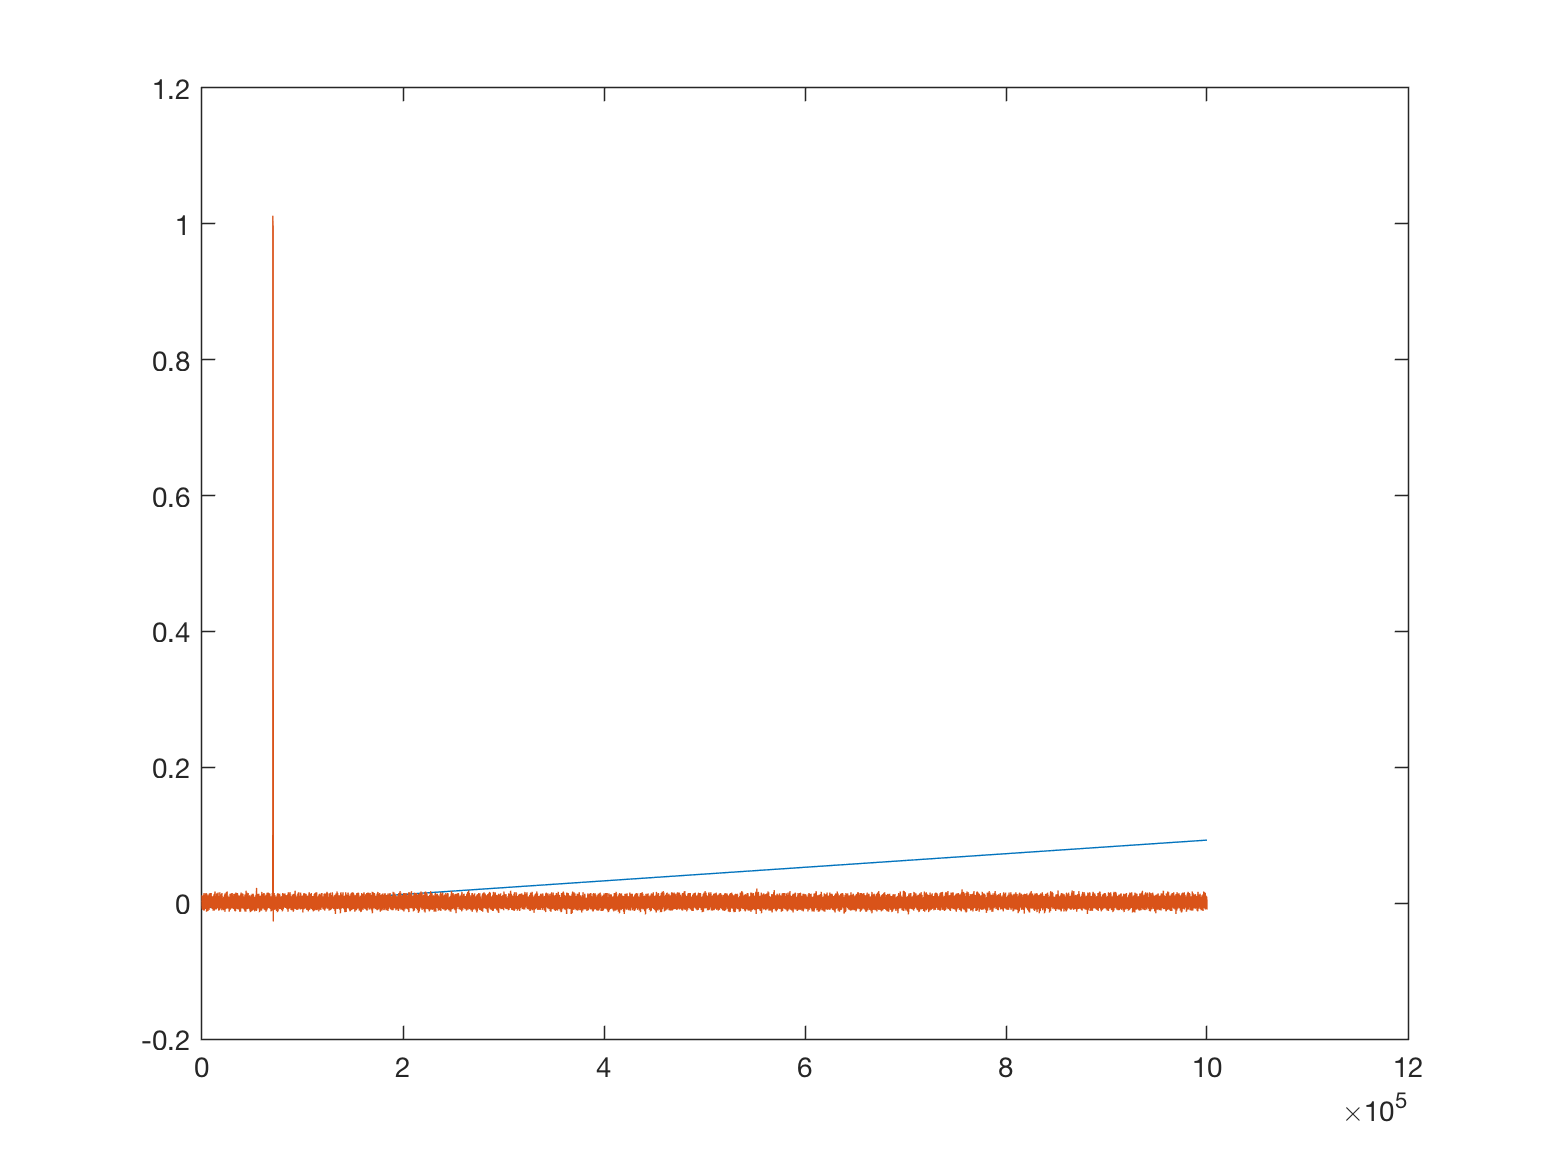
\includegraphics[width=0.9\textwidth, height=5cm]{billeder/reverb_input.png}
		\caption{Input på reverbtesten.}
	\end{minipage}\hfill
	\begin{minipage}{0.50\textwidth}
		\centering
		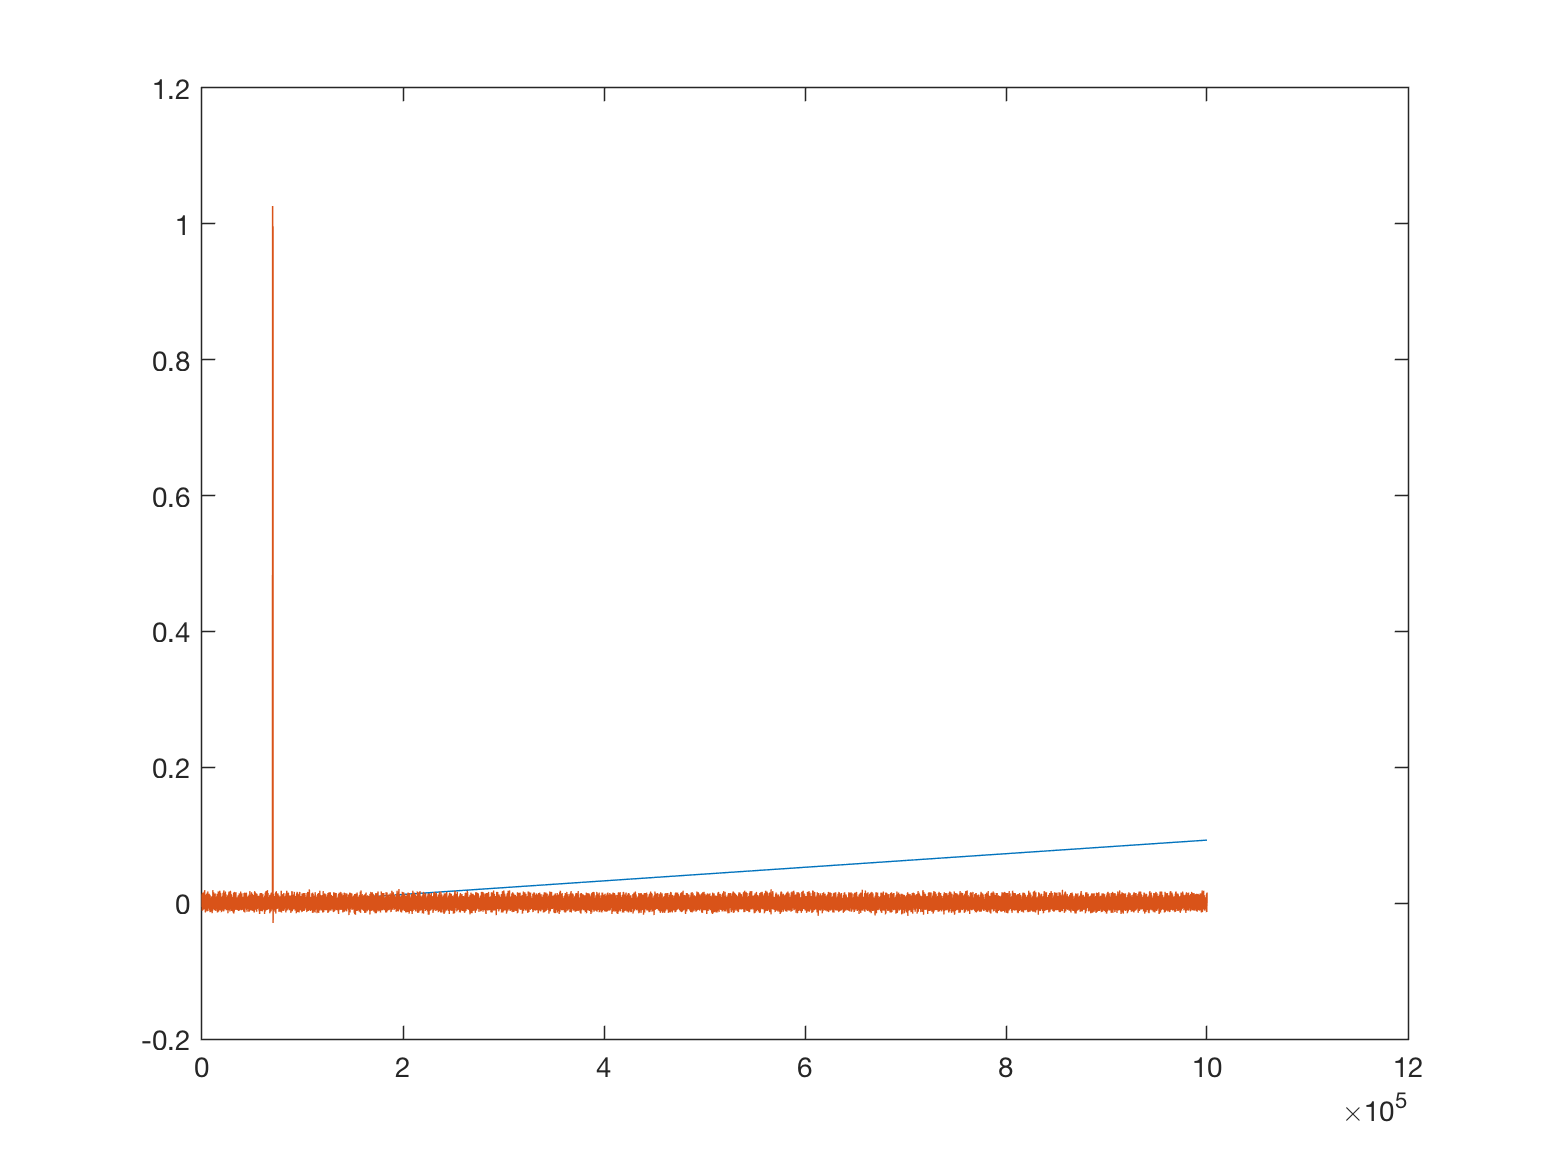
\includegraphics[width=0.9\textwidth, height=5 cm]{billeder/echo_input.png}
		\caption{Input på echotesten.}
	\end{minipage}
\end{figure}
\husk{Sonny}{kan godt huske noget om at vi også testede på indgange til µControlleren, men var der ikke den samme støj på den almindelige indgang og vi ser den næsten heller ikke i matlab plottende}
Støjen på indgangen skyldes de tre anti-aliasing filtre, som var forbundet via \husk{hvad kalder man de ting} hvilket giver en dårlig forbindelse.\newline
\begin{figure}[!ht]
	\centering
	\begin{minipage}{0.50\textwidth}
		\centering
	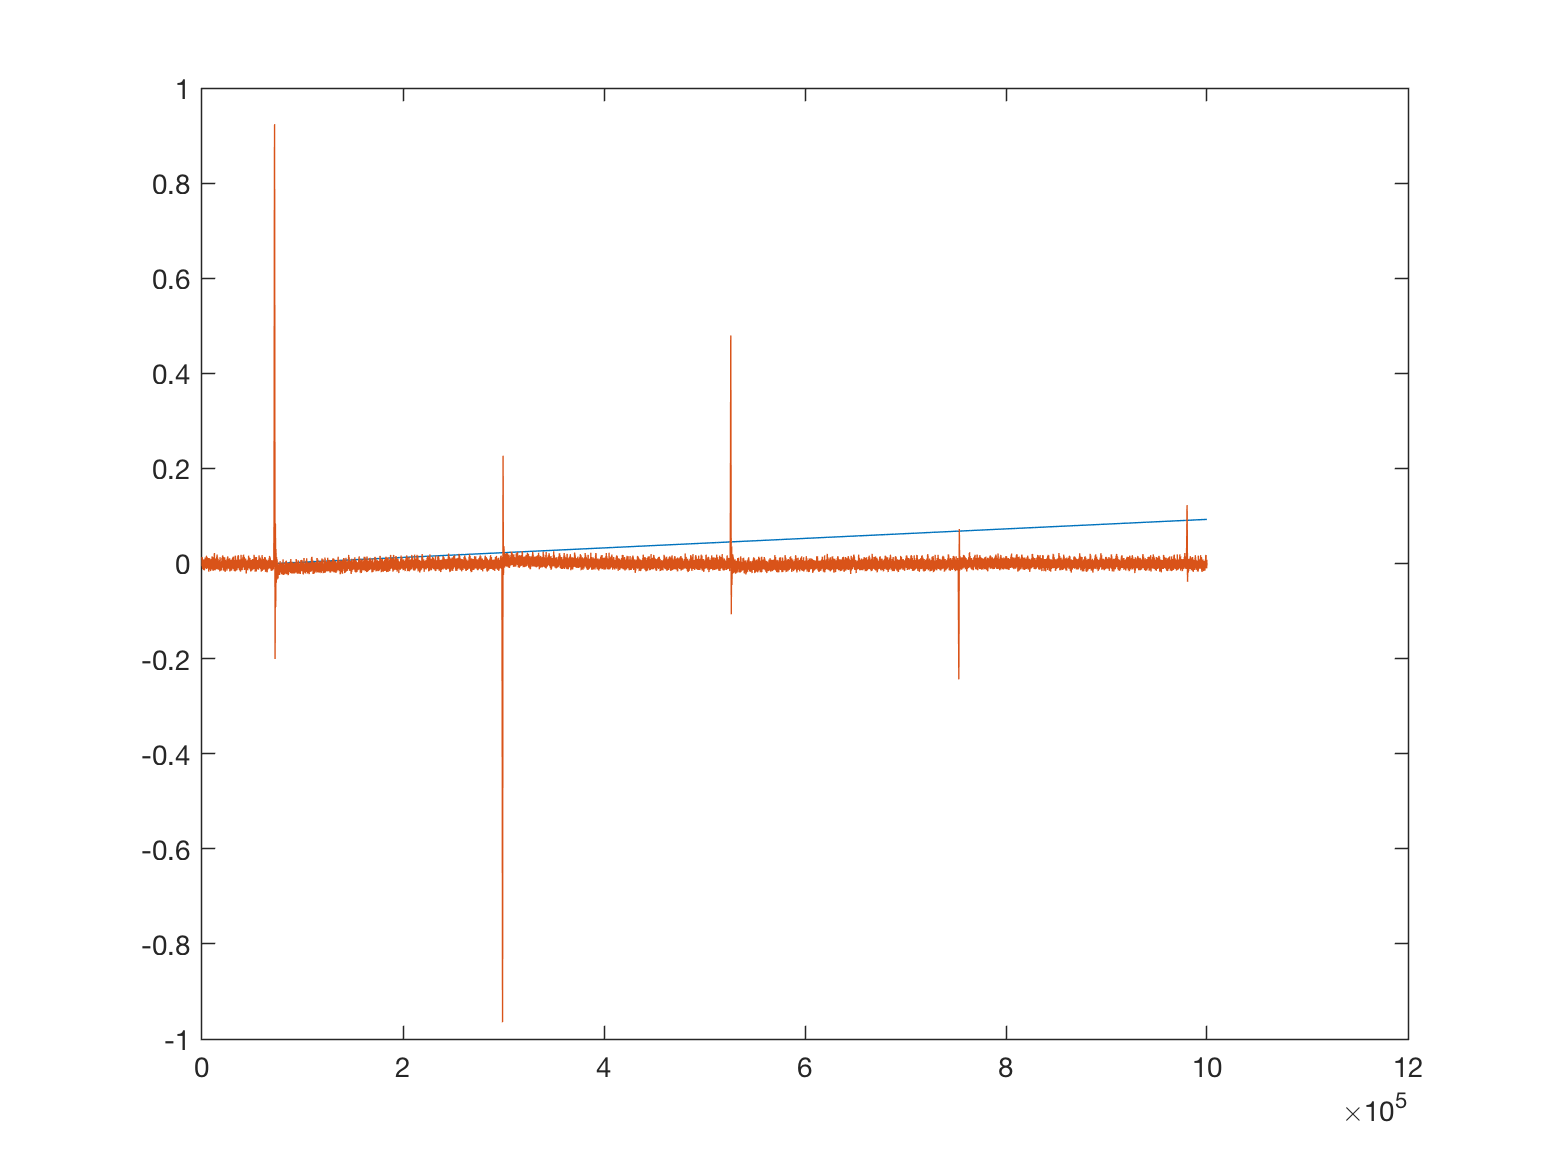
\includegraphics[width=0.9\textwidth]{billeder/reverb_res.png}
	\caption{Impulsrespons af reverb}
	\label{fig:impulsresponsreverb}
	\end{minipage}\hfill
	\begin{minipage}{0.50\textwidth}
		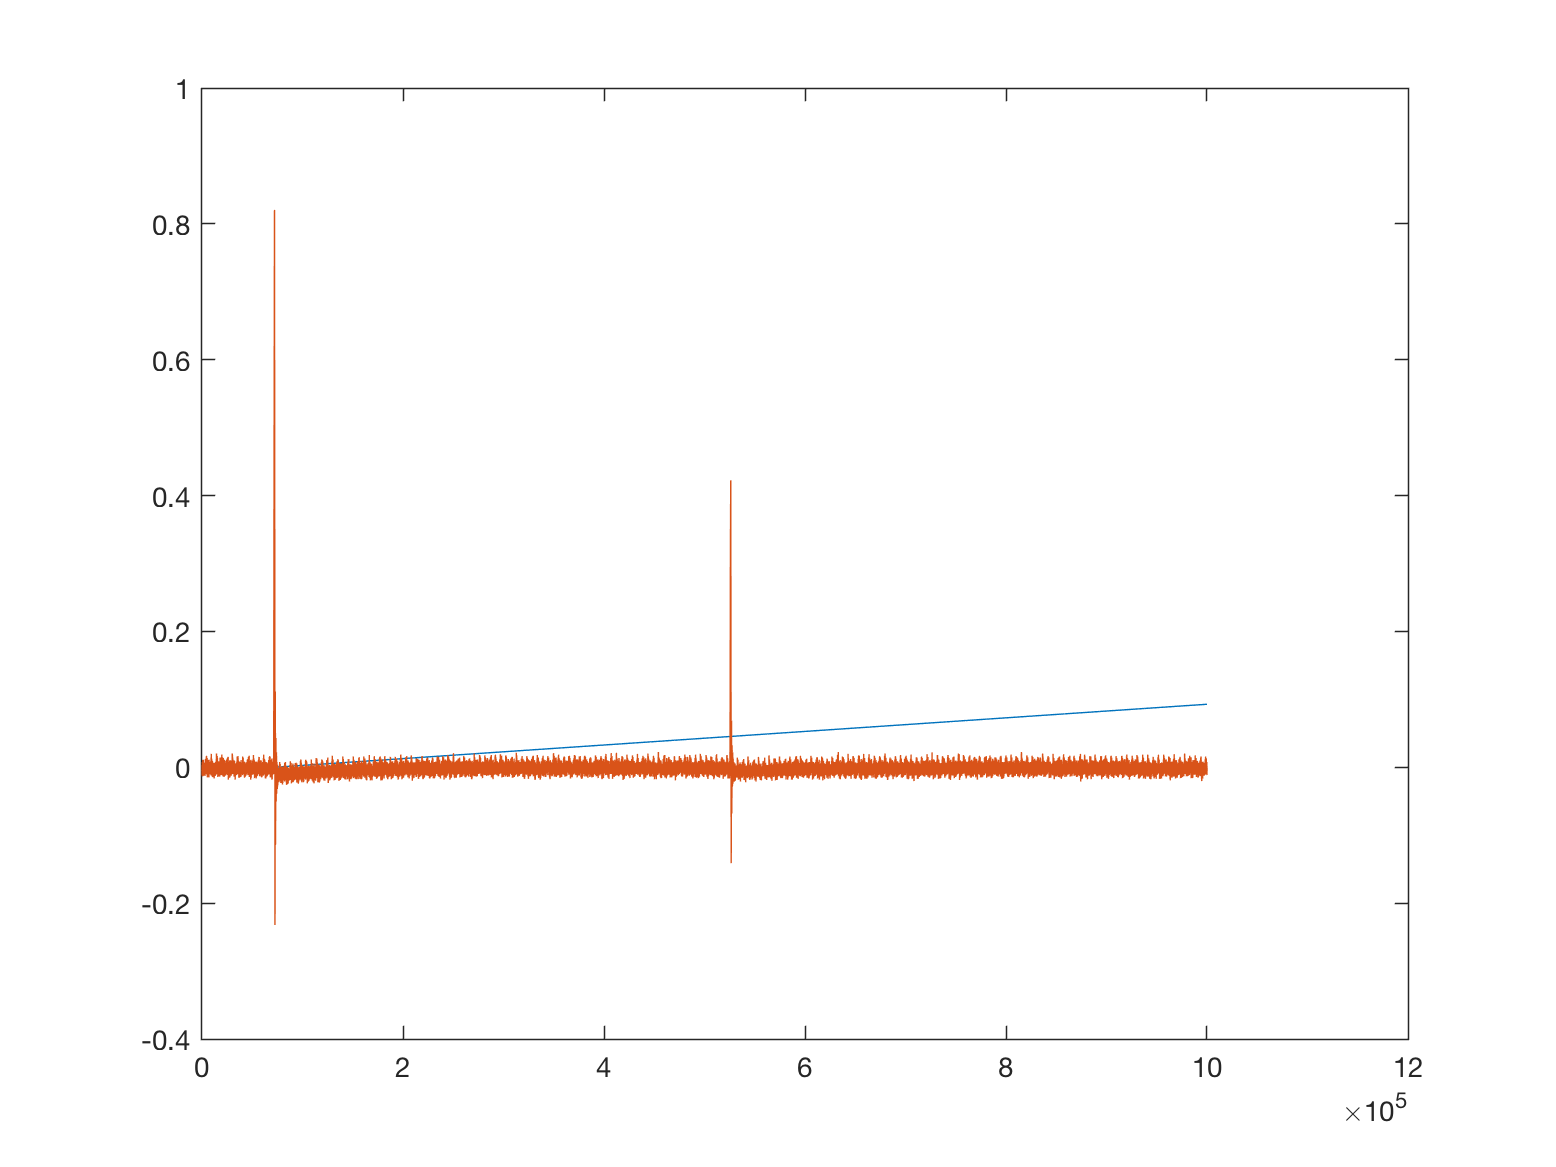
\includegraphics[width=0.9\textwidth]{billeder/echo_res.png}
		\caption{Impulsrespons af echo}
		\label{fig:impulsresponsecho}
		\end{minipage}
\end{figure}
\husk{Sonny}{Først målte tal så hvad de tilsvare præcis i "samples" og så kan der siges at det passer til det delay vi forventede}
Her \ref{fig:impulsresponsreverb} ses impulsresponset af reverbeffekten.
Som det fremgår af figuren bliver samplen gengivet med en dæmpning hver $2000$. sample.
Gains samt delay var sat højt for at overdrive og tydeliggøre feedbacket.\newline
Som det ses på figuren bliver impulsen feedbacket èn gang som svarende til et ekko efter $2000$ svarende til $45,35\si{mS}$.

